\section{Discussion of Results}\label{sec:result}
    
\subsection{Evaluation Against Other Approaches}

\begin{figure}
    \includegraphics[width=\linewidth]{analysis/artefact/variation_approach/reduction_query_execution_time}
    % General caption
    \caption{
    Comparison of query execution time with the type index approach.
    The ratio represents how the execution time of each method compares to that of the type index. 
    A ratio greater than $1$ indicates a slower execution time (\textbf{lower is better}).
    The shape index approach performs similarly or better than the other methods, except in the case of S4.
    }
    \label{fig:compApproach}
\end{figure}

Figure~\ref{fig:compApproach} shows that the shape index approach performs better or comparably to the state-of-the-art Solid Pod network traversal algorithms, for all query templates except S4.
Figure~\ref{fig:compApproachRaw} in the \hyperref[sec:appendix]{Appendix} present the execution time of each method.
An analysis of statistical significance is provided in the \hyperref[sec:supplementalMaterial]{supplementary material}.
Moreover, the shape index approach allows for answering queries from the S7 template, which was not possible by the other approaches, due to large amount of HTTP requests resulting in timeouts.
Queries can require as little as 13\% of the execution time (S1 being 7 times faster) of the type index.
The queries that perform the best are those in which the number of HTTP requests decreased the most, as can be inferred from the analysis of Table~\ref{tab:ratioUsefulResources}.
Table~\ref{tab:ratioUsefulResources} presents the average percentage of query-relevant resources per query template, derived from the where-provenance~\cite{buneman2001and} of the query results and the number of HTTP requests. 
%Table~\ref{tab:statSignificanceStateOfTheArt} presents an analysis of the statistical significance of the query template and its relation to the ratio of HTTP requests performed.
Queries from templates D6 and D7 show no reduction because they require nearly every document in the dataset to be processed by the engine, making our approach ineffective in these cases.
We notice that queries from template S4 with the shape index performed worse in every instance, with an increase in query execution time of up to 2.80 times.
This is further illustrated in Table~\ref{tab:ratioUsefulResources}, which shows that for these queries, the type index traversal algorithm achieves a ratio of useful resources dereferenced of 100\% or 50\%, compared to only 6\% with the shape index approach.
The poor performance is due to the fact that the links acquired by the other approaches were selected based on reachability criteria that did not leverage the structural properties of the dataset, such as in the case of \texttt{Cmatch}~\cite{hartig2016walking} (a reachability criterion based on the structure of the query).
In contrast, the shape index approach always enforces the use of these properties, resulting in additional HTTP requests and increased processing time.
%It has to be highlighted that our formalization assumes that structural assumptions are always used and that the shape index, if present, will be part of the traversal, see section~\ref{sec:sourceSelection}.
However, those queries were already fast, with the type index traversal algorithm approach being executed in approximately 0.30\% of the maximum execution time allowed.
Nonetheless, these results still highlight a category of queries and networks for which our approach is not well-suited.
Those results mostly validate \textbf{H1} however the shape index approach can drastically increase the execution time when the structural properties are not used.

\input{analysis/artefact/ratio_useful_resources/table_ratio_useful_resources_summary} 


To further our analysis, we compare three temporal metrics: the arrival time of the first results, the termination time, defined as the duration between the arrival of the last result and the end of query execution, and the waiting time, which we define as the accumulated time gaps exceeding one second between the reception of consecutive results.
We choose a 1 second threshold for waiting time based on research in responsive system design.
These guidelines are derived from the field of neuropsychology and are considered stable over time for human users~\cite{uxtigersNeedSpeed, Nielsen1993}.
A waiting time below 0.1 seconds is perceived as instantaneous, a delay of up to 1 second preserves a seamless flow of thought, while delays exceeding 10 seconds tend to cause user attention to drift~\cite{Nielsen1993}.
We additionally computed the diefficiency metric in relation to time (\textit{dief@t})~\cite{Acosta2017}, at the previously mentioned time intervals: 0.1\,s, 1\,s, and the arrival time of the final result.
We did not choose 10\,s as the threshold, since all queries that terminate complete in under 10\,s.
Tables~\ref{tab:continuousPerf} and \ref{tab:dief} in the \hyperref[sec:appendix]{Appendix} present the average results for the metrics presented above.


\begin{figure}
    \centering
    \includesvg[width=\linewidth]{analysis/artefact/continuous_performance/first_result}
    \caption{The shape index approach tends to produce the first results earlier than the type index approach, particularly for queries where the shape index achieves shorter total execution times.}
    \label{fig:first_res}
\end{figure}

Figure~\ref{fig:first_res} presents the time of arrival of the first results for all query instances, grouped by query templates. 
The plot indicates that, for most queries, the shape index approach tends to produce results faster, as shown by distributions concentrated around lower first result arrival times.
Templates D1, D2, D5, and S1 exhibit the most significant improvements in first-result latency when using the shape index.
However, as shown in Figure~\ref{fig:compApproach}, some instances of queries from templates D2 and D5 perform worse under the shape index compared to the type index approach.
Nevertheless, particularly for D5, the overall distribution remains significantly lower.
This suggests that, although the shape index does not explicitly prioritize early result generation, the pruning it performs may implicitly favor certain faster first results arrival with some query and network. 
This implicit prioritization does not apply uniformly across all templates. 
For example, queries from template D3 show faster overall execution times across most instances, yet in Figure~\ref{fig:first_res}, they exhibit a higher mean and a longer tail for the first result arrival time.
Notably, the most prominent mode in the distribution under the type index lies at a lower first-result time compare to the shape index.
This can be explained by the structure of the subwebs involved in D3 queries.
In some cases, a result can be generated from a document that is only one link away from the seed document.
The direct dereferencing used by the type index enables this early discovery.
In contrast, the shape index may delay first result production due to its reliance on document discovery to perfrom the pruning operations.


\begin{figure}
    \centering
    \includesvg[width=\linewidth]{analysis/artefact/continuous_performance/termination_time}
    \caption{With the exception of queries from templates D6 and D7, which have similar execution times, the shape index either maintains or improves query termination time.}
    \label{fig:termination_time}
\end{figure}

Figure~\ref{fig:termination_time} present the termination time for the query execution instances, grouped by templates.
It shows that for queries where the execution time was improved and where the termination time was not close to 0 such has queries from the template D1, S1 and S5, 
the shape index approach can decrease significantly the termination time.
In the case of queries from the template D6 and D7 the distribution have a similar shape but a longer tail.
Particularly D7 which can approximatively take up to one second more to terminate.

... Let's find an explication......


\begin{figure}
    \centering
    \includesvg[width=\linewidth]{analysis/artefact/continuous_performance/waiting_time}
    \caption{Except for queries from template D1, the shape index approach tends to either maintain or worsen the waiting time.}
    \label{fig:waiting_time}
\end{figure}

Figure~\ref{fig:waiting_time} presents the waiting time for the query instances, grouped by template. 
With the exception of queries from dataset D1, which show a decrease in waiting time, the shape index approach generally increases the waiting time for queries that experience a delay before producing results. 
A likely explanation for this increase is the additional time required to dereference documents related to the shape index, which may introduce a gap before the production of results, even though the total query execution time is reduced or remains unchanged.


\begin{figure}
    \centering
    \includesvg[width=\linewidth]{analysis/artefact/continuous_performance/dief_1}
    \caption{At 1 second, the shape index approach shows a higher \textit{dief@1s} (\textbf{higher is better}), indicating that more results are obtained while maintaining a seamless flow of thought.}
    \label{fig:dief_1}
\end{figure}

Figures~\ref{fig:dief_1} and~\ref{fig:dief_lr} show the \textit{dief@t} values measured at 1 second (\textit{dief@1s}) and at the time of the last result produced for all evaluated approaches (\textit{dief@lr}).~\footnote{This means that if, for a given query, the shape index approach produces the last result at 5~seconds and the type index at 5.10~seconds, then the \textit{dief@t} metric will be computed at 5.10~seconds.}
The \textit{dief@1s} results indicate that the shape index approach generally produces a higher number of early results, except for queries from templates S4 and S5.
Which indicate that for fast result arrival the shape index approach performs better.
This result is important in the context of social media applications where it is often not necessary to get fast complete results, but to get a fast relevant results to keep interactivity.



In contrast, the \textit{dief@lr} values show that the shape index performs similarly than the type index approach exept for D4 where it performs better,

except for template D4, even in cases where the overall query execution time is significantly reduced.
One reason for the relative drop in performance from \textit{dief@1s} to \textit{dief@10s} is that all queries complete that finish before the timeout are executed  in less than 10 seconds.
Since \textit{dief@t} measures the area under the curve of cumulative results over time, calculating it after the final result has been produced means both approaches tend to converge to similar values.
As a result, differences between the methods diminish as $t$ increases beyond the query completion time.

% Maybe we should plot dief@lastResultTime

\begin{figure}
    \centering
    \includesvg[width=\linewidth]{analysis/artefact/continuous_performance/dief_lr}
    \caption{At the time of the last result, the shape index approach tends to exhibit a similar \textit{dief@t} (\textbf{higher is better}).}
    \label{fig:dief_lr}
\end{figure}

\subsection{Query-Shape Subsumption Evaluation} \label{sec:experimentAlgoSubsumption}

The empirical evaluation of the query-shape subsumption algorithm shows that its execution time with the more detailed shapes from our experiment is negligible, with a maximum execution time of 4.655 ms (0.0039\% of the timeout).
The result tables are available in the \hyperref[sec:supplementalMaterial]{supplementary material}.
This outcome is expected, as the algorithm has polynomial time complexity, and the shapes and queries in the experiments are small and not deeply nested.
This result validated \textbf{H2}.


\subsection{Evaluation of the Resilience of the approach}

The final part of the results analysis focuses on the resilience of the shape index approach.
In this analysis, we examine the impact of reducing the shape index information in the network and compare the results with a network in which all pods are exposed to detailed, complete shape indexes.
Figure~\ref{fig:adaptShapeIndex} presents three plots that illustrate the results of our evaluation of the approach's resilience.
The plot on the left shows the variation in the availability of shape indexes across the network. 
As expected, we observe that queries that performed better in Figure~\ref{fig:compApproach} tend to perform worse with reduced shape index information, while queries that performed poorly improved. 
%Queries that were unaffected by the shape index changes remain unaffected.


\begin{figure}
    \centering
    \includegraphics[width=1\linewidth]{analysis/artefact/variation_shape_index_all/plot}
    \caption{
    Shape index approaches tend to perform less effectively with limited network information and comparatively better where the baseline shape index underperforms.
    A higher ratio indicates a longer query execution time compared to a network with complete shape index information (\textbf{lower is better}).
    %However, the utility of shape index information can vary depending on the specific queries and network characteristics.
    }
    \label{fig:adaptShapeIndex}
\end{figure}


The plot in the middle shows the variation in the percentage of shape index entries using closed shapes.
The results here are more nuanced.
While there is a general trend for query evaluations with a lower percentage of closed shapes to behave similarly to the plot on the left, we also observe both performance gains for some query template and a drastic performance loss for the queries of S1 when 80\% of the shape entries are closed.
The performance gain occurs because not every entry needs to be closed to prune the query irrelevant documents.
Entries mapped to an open shape are always considered relevant because the shape translates to a query fetching the whole KG.
If the subsumption check leads to the same conclusion, then, given a closed entry, the execution will be more expensive because 
when shapes are nested, the nested shapes need to be dereferenced to solve the query-shape subsumption algorithm.
For the queries of S1, with 80\% of closed shape entries, the performance lost was due to random chance, as the discriminatory entries were provided with open shapes in multiple instances when looking at the raw data.

The right plot shows the variation in the level of detail of the shapes by reducing their detail.
Since the shapes are closed in this experiment the level of detail was varied by changing the constraint of the object terms of the shape as described in Section~\ref{sec:experiment}.
Most queries tend to perform similarly or better, with the exception of those of S1.
Upon analyzing the output of our query subsumption algorithm, we observe that the additional information to the shape provided in our base approach does not affect the algorithm's results.
However, in the baseline shape index experiment, the engine must dereference more shapes, potentially increasing execution time.
Queries of template S1 are the only ones where the added information can discriminate multiple parts of the datasets' domain leading to worse performane.
This indicates that in some situations, adding more information can be beneficial.
This sensitivity of the quantity of the information in the index also helps explaining the results for S1 queries in the middle plot. 
In that case, the engine still had to dereference shapes from each dataset, and the information available was likely insufficient to significantly discriminate between resources.

These results show that \textbf{H3} and \textbf{H4} are rejected: reducing information is not always detrimental to query execution.
It becomes detrimental only when the omitted information is critical for determining the query relevance of resources. 
Therefore, the outcome is dependent on both the query and the network. 
Moreover, the completeness of shape indexes has a smaller impact on performance than their presence or absence.
\textbf{H5} is accepted; it is possible to retain performance gains even in networks with reduced shape-index information.

\begin{figure}[htbp]
    \centering
    % First figure
    \begin{minipage}[t]{0.45\linewidth}
        \centering
        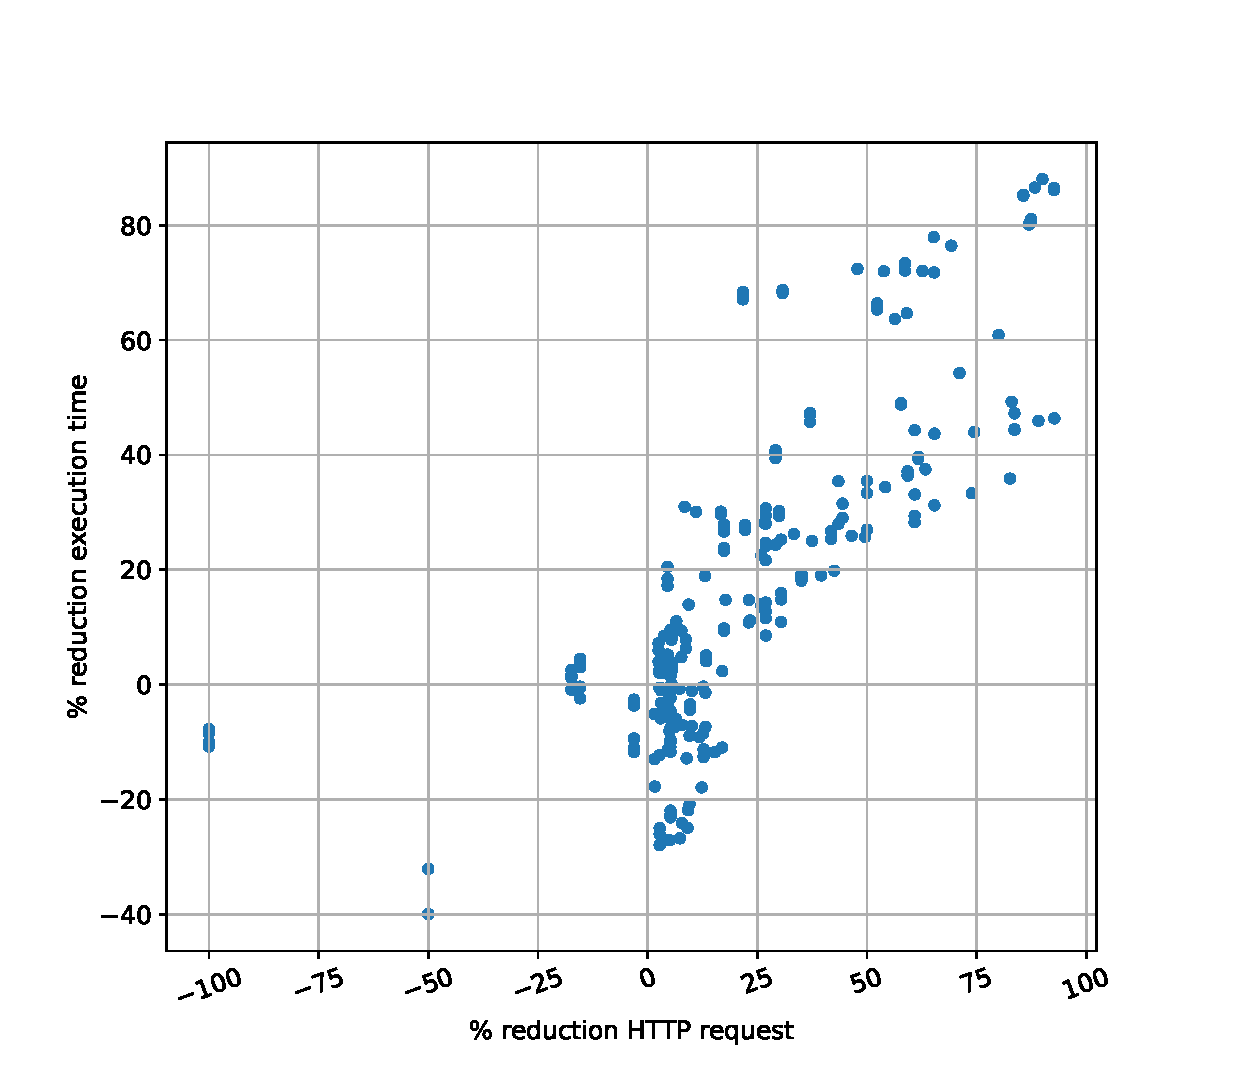
\includegraphics[width=\linewidth]{analysis/artefact/http_req_exec_time_relation/http_req_exec_time_cor_better}
        \label{fig:http_req_exec_time_cor_better}
    \end{minipage}
    \hspace{0.05\textwidth}
    % Second figure
    \begin{minipage}[t]{0.45\linewidth}
        \centering
        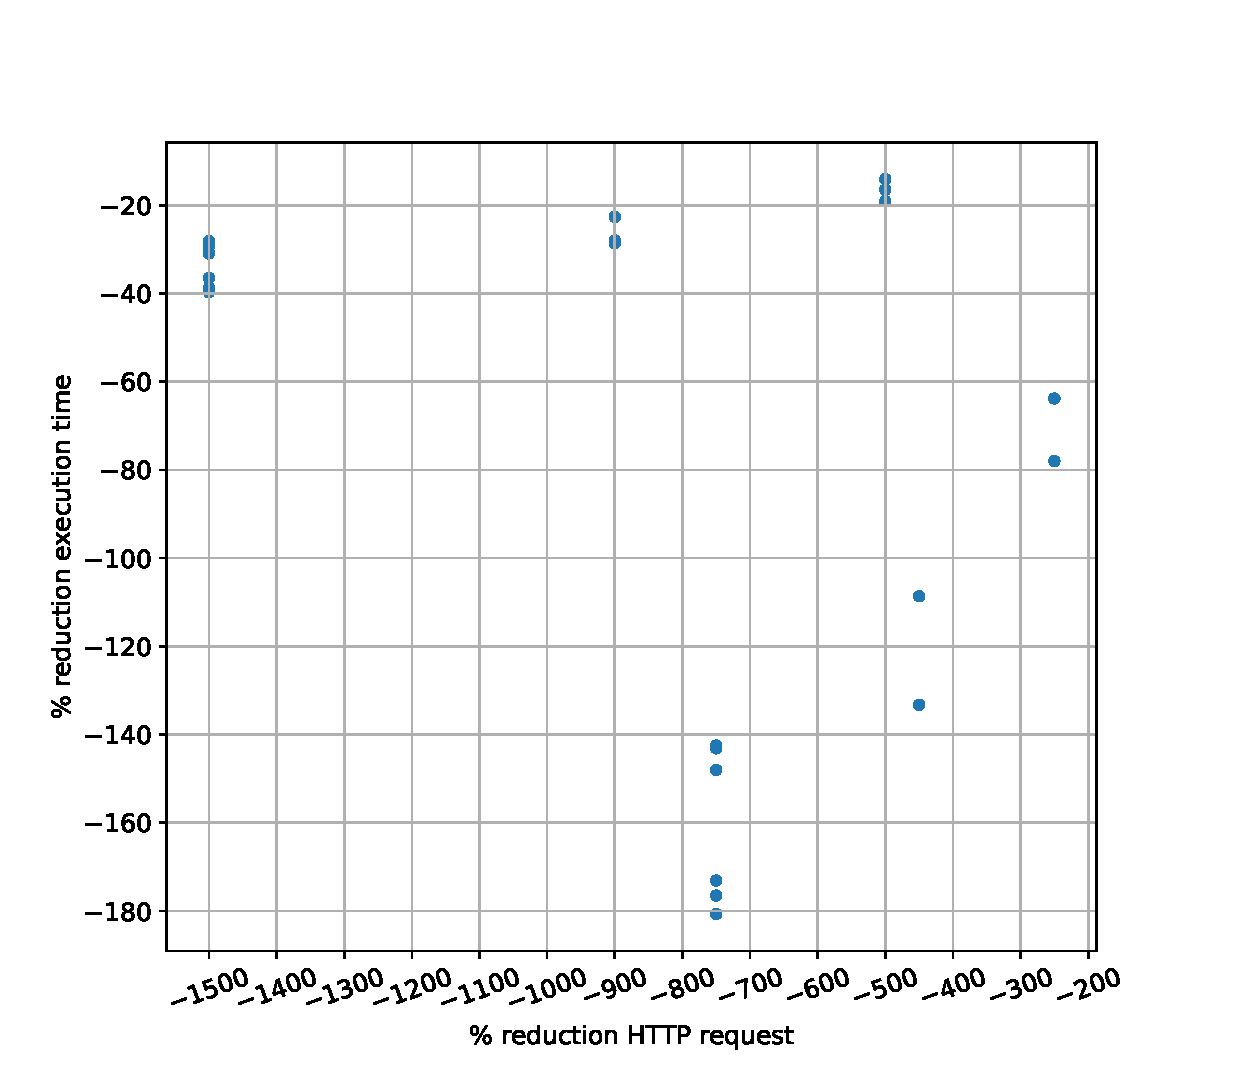
\includegraphics[width=\linewidth]{analysis/artefact/http_req_exec_time_relation/http_req_exec_time_cor_worse}
        \label{fig:http_req_exec_time_cor_worse}
    \end{minipage}

    % General caption
    \caption{
        The data show two regimes in the relation between the number of HTTP requests and the execution time, 
        we see a more linear correlation on the left figure than on the right figure.
        }
    \label{fig:http_req_exec_time_cor}
\end{figure}

\subsection{Relationship Between HTTP Request and Query Execution Time}


To study the relationship between the number of HTTP request and the query execution time, the ratio of HTTP request of the different approaches and the ratio of query execution time was 
calculated in relation to the Solid Pod network traversal algorithms leveraging the type index.
Figure~\ref{fig:http_req_exec_time_cor} present our analysis.
The relationship between HTTP request and query execution time can be divided into two regimes.
In the first regime (left figure), where the shape index approach reduces the number of HTTP requests, we notice a positive linear correlation with a Pearson correlation coefficient (PCC) of 0.84 and a high statistical significance ($< 0.01$).
We can notice that toward the end, the curve appears to exhibit a more exponential behavior.
Evaluating an $R^2$ score with an exponential best fit curve we get a score of 0.72 and 0.71 for a linear curve.
Above a ratio of approximately 0.85 of HTTP requests, the shape index approach did not guarantee a reduction in query execution time.
There can be multiple explanation for this behavior.
First, the method have some overhead due to the query-shape subsumption algorithm and the state retention of the pruning reachability criteria.
However, as shown in in section \ref{sec:experimentAlgoSubsumption} the query-shape subsumption algorithm execution time is negligeable for one execution and the state retentation has a polynomial time complexity thus it should not have a high impact on the execution time.
Another explanation is the number of HTTP request that are performed in parallel.
The LTQP version of comunica perform 10 HTTP requests in parallel, thus we would expect that with a low number of HTTP request perform and a low ratio of HTTP request that the performance would remain unchanged or a little bit worse due to some overhead which is what 
can be withness in the curve.

In the second regime (right figure), the shape index increases the number of HTTP requests.
We notice a moderate positive linear correlation with a PCC of 0.44.
The overall correlation between reducing HTTP requests and query execution time is positively linear, with a moderate linear correlation with a PCC of 0.56 and a high statistical significance.
The overall correlation is more linear than exponential with $R^2$ scores respectively of 0.31 and 0.24, however due to the low score it is difficult to determine the nature of the distribution.

Explaining the two behavioral regimes observed in the data is challenging.
One possible explanation for the poorer performance of the shape index approach in certain cases could be the low number of samples.
However, we also observe that the relationship between the two variables differs significantly across the regimes.
In the first regime, the relationship is close to one-to-one, with a slope of approximately 0.91.
In contrast, the second regime shows a much flatter slope of around 0.08, suggesting that the ratio of HTTP requests has a weaker influence.
This disparity indicates that the explanation may be more complex than just a sample size issue.
The increased number of HTTP requests can be attributed to queries executed using the D6, D7, and S4 templates, with the S4 template causing the largest increase.
Queries from the S4 template typically require only 1 or 2 HTTP requests, so when running with 10 concurrent requests, the impact on performance is limited.
On the other hand, queries using the D6 and D7 templates, executed with the type index traversal algorithm, required 26, 23, and 129 HTTP requests.
This significantly higher number of HTTP requests explains why the increase in HTTP requests had a greater impact on query execution time.

These results partially validate \textbf{H6}, as a linear relationship is observed when there are a sufficient number of HTTP requests and a significant reduction ratio, taking concurrent requests into account.